\documentclass{beamer}
\usepackage[latin1]{inputenc}
\usepackage{times}
\usepackage{tikz}
\usetheme{Luebeck}
%\usecolortheme{albatross}
\usepackage{amsmath,amsfonts,amsthm,amssymb}
\usepackage{setspace}
\usepackage{Tabbing}
\usepackage{fancyhdr}
\usepackage{lastpage}
\usepackage{extramarks}
\usepackage{chngpage}
\usepackage{soul,color}
\usepackage{graphicx,float,wrapfig}
\usepackage{xcolor}
\usepackage{listings}
\usepackage{float}
%\usepackage{subfloat}
\usepackage{subfig}
\usepackage{caption}
\usepackage{enumitem}
\usepackage{algpseudocode}

\definecolor{darkorange}{RGB}{240, 120, 0}
\definecolor{darkgreen}{RGB}{0, 128, 0}

\setbeamercolor{background canvas}{bg=white}
\setbeamercolor{frametitle}{fg=white, bg=darkorange}
\setbeamercolor{normal text}{bg=black,fg=black}
\setbeamercolor{structure}{bg=black, fg=darkorange}

\title{Lecture 6: Normal Transformations, 3D Transformations, Euler Angles}
\date{2/2/2016}
\institute{Chris Tralie, Duke University}
\author{COMPSCI/MATH 290-04}
\begin{document}

\frame{\titlepage}

\begin{frame}{Announcements}

\begin{itemize}[label=$\blacktriangleright$]
    \item Mini Assignment 2 Out, Due Next Monday 11:55 PM
    \item Online notes coming soon... (for now slides)
\end{itemize}

\end{frame}

\begin{frame}{Table of Contents}

\begin{itemize}[label=$\blacktriangleright$]
	\item Linear Functions Continued
\end{itemize}
\begin{itemize}[label=$\vartriangleright$]
	\item Normal Transformations
	\item Linear Equations
    \item 3D Transformations / Euler Angles
\end{itemize}

\end{frame}



\begin{frame}{Column Vector Walking Interpretation}

\[
\left[ \begin{array}{cccccc} | & | & \vdots & | & \vdots & | \\ \vec{v_1} & \vec{v_2} & \hdots & \vec{v_k} & \hdots & \vec{v_N} \\ | & | & \vdots & | & \vdots & | \end{array}  \right] \left[ \begin{array}{c} 0 \\ 0 \\ \vdots \\ a_k \\ \vdots \\ 0 \end{array} \right] = a_k \vec{v_k}
\]

\end{frame}


\begin{frame}{Column Vector Walking Interpretation}

\[
\left[ \begin{array}{cccc} | & | & \vdots & |\\ \vec{v_1} & \vec{v_2} & \hdots & \vec{v_N} \\ | & | & \vdots & | \end{array}  \right] \left[ \begin{array}{c} a_1 \\ a_2 \\ \vdots \\ a_N \end{array} \right] = \sum_{i=1}^{N} a_i \vec{v_i}
\]

Linear combination of column vectors!

\end{frame}



\begin{frame}{Column Vector Walking Interpretation}

\[ \left[ \begin{array}{cc} \textcolor{red}{-1} & \textcolor{blue}{1} \\ \textcolor{red}{0} & \textcolor{blue}{1} \end{array} \right]   \left[ \begin{array}{c} u \\ v \end{array} \right]  = \left[ \begin{array}{c} \textcolor{red}{-1} \\ \textcolor{red}{0} \end{array} \right] u + \left[ \begin{array}{c} \textcolor{blue}{1} \\ \textcolor{blue}{1} \end{array} \right] v \]

\begin{figure}[t]
	\centering
    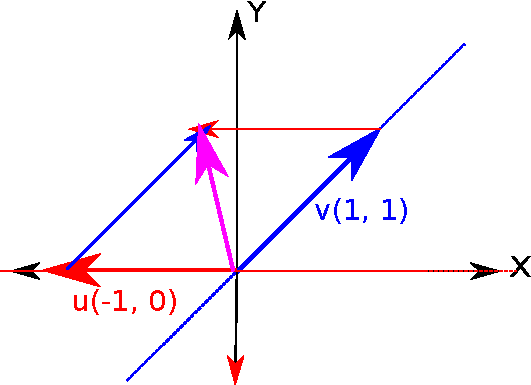
\includegraphics[width=0.7\textwidth]{ColumnVectorAdd.pdf}
\end{figure}


\end{frame}


\begin{frame}{Linear Function To Matrix Proof}
\begin{itemize}[label=$\vartriangleright$]
\item Define a linear function $L: x \in \mathbb{R}^N \rightarrow y \in \mathbb{R}^M$
\end{itemize}


\uncover<2->{
\begin{itemize}[label=$\vartriangleright$]
\item Let $L^j$ = $L \left( \left\{ \begin{array}{cc} 1 & k = j \\ 0 & \text{otherwise} \end{array} \right\}, k = 1\text{ to }N \right)$
\end{itemize}
}

\uncover<3->{
\[
\left[ \begin{array}{cccc} | & | & \vdots & |\\ L^1 & L^2 & \hdots & L^N \\ | & | & \vdots & | \end{array}  \right] \left[ \begin{array}{c} a_1 \\ a_2 \\ \vdots \\ a_N \end{array} \right] = \sum_{i=1}^{N} a_i L^i
\]
}

\uncover<4->{
\begin{itemize}[label=$\vartriangleright$]
\item Recall that for a linear function: $L(ax + by) = aL(x) + bL(y)$
\end{itemize}
}


\end{frame}

\begin{frame}{Linear Function To Matrix Example}

\[ f(x, y, z) = (x + y + 2z, 3x - 2y) \]

\[ f(1, 0, 0) = \]

\[ f(0, 1, 0) = \]

\[ f(0, 0, 1) = \]

\end{frame}

\begin{frame}{Square Matrix Inverse}

\[ A^{-1}A = I \]
\[ AA^{-1} = I \]

\uncover<2->{
Example:

\[ A = \left[ \begin{array}{cc} 2 & 0 \\ 0 & 1 \end{array} \right], A^{-1} = \left[ \begin{array}{cc} 0.5 & 0 \\ 0 & 1 \end{array} \right] \]
}

\end{frame}


\begin{frame}{Square Matrix Inverse}

\[ A^{-1}A = I \]
\[ AA^{-1} = I \]

Example:
\[ A = \left[ \begin{array}{cc} -1 & 0 \\ 0 & 1 \end{array} \right], A^{-1} = \left[ \begin{array}{cc} -1 & 0 \\ 0 & 1 \end{array} \right] \]

\end{frame}


\begin{frame}{Square Matrix Product Inverse}

\[ (AB)^{-1} = B^{-1}A^{-1} \]
\end{frame}


\begin{frame}{Matrix Transpose}

\[ A^T_{ij} = A_{ji} \]

$A: M\times N \iff A^T: N\times M$

\uncover<2->{
\[
A = \left[ \begin{array}{cccccc} | & | & \vdots & | & \vdots & | \\ \vec{v_1} & \vec{v_2} & \hdots & \vec{v_k} & \hdots & \vec{v_N} \\ | & | & \vdots & | & \vdots & | \end{array}  \right]
\]
}

\uncover<3->{
\[
A^T = \left[ \begin{array}{ccc} - & \vec{v_1} & - \\ - & \vec{v_2} & - \\ \vdots & \hdots & \vdots \\ - & \vec{v^N} & - \end{array}  \right]
\]
}

\end{frame}

\begin{frame}{Matrix Transpose Example}

\[ A = \left[ \begin{array}{cccc} 1 & 2 & -2 & 3 \\ 0 & 4 & 5 & -1 \\ 6 & -4 & 3 & 2 \end{array} \right] \]
\[ A^T = \left[ \begin{array}{ccc} 1 & 0 & 6 \\ 2 & 4 & -4 \\ -2 & 5 & 3 \\ 3 & -1 & 2 \end{array} \right] \]

\end{frame}

\begin{frame}{Transpose of Product Matrix}

\[ (AB)^T = B^TA^T \]

Check dimensions!

\end{frame}


\begin{frame}{Rotation Matrices Inverse}

\[ R_{\theta} = \left[ \begin{array}{cc} \cos(\theta) & -\sin(\theta)\\ \sin(\theta) & \cos(\theta) \end{array} \right] \]

\uncover<2->{
\[ R^{-1}_{\theta} = R_{-\theta} = \left[ \begin{array}{cc} \cos(\theta) & \sin(\theta)\\ -\sin(\theta) & \cos(\theta) \end{array} \right] \]
}

\uncover<3->{

\[ R^{-1}_{\theta} = R^T_{\theta} \]

}

\end{frame}


\begin{frame}{Table of Contents}

\begin{itemize}[label=$\vartriangleright$]
	\item Linear Functions Continued
\end{itemize}
\begin{itemize}[label=$\blacktriangleright$]
	\item Normal Transformations
\end{itemize}
\begin{itemize}[label=$\vartriangleright$]
    \item Linear Equations
    \item 3D Transformations / Euler Angles
\end{itemize}

\end{frame}



\begin{frame}{Normal Transformations}

\[ \left[ \begin{array}{cc} \cos(\theta) & -\sin(\theta)\\ \sin(\theta) & \cos(\theta) \end{array} \right] \left[ \begin{array}{c} x \\ y \end{array} \right] =  \left[ \begin{array}{c} x \cos(\theta) - y\sin(\theta) \\ x \sin(\theta) + y\cos(\theta) \end{array} \right] \]

\begin{figure}[t]
    \captionsetup[subfloat]{labelformat=empty}
	\centering
	\subfloat[Before]{
	    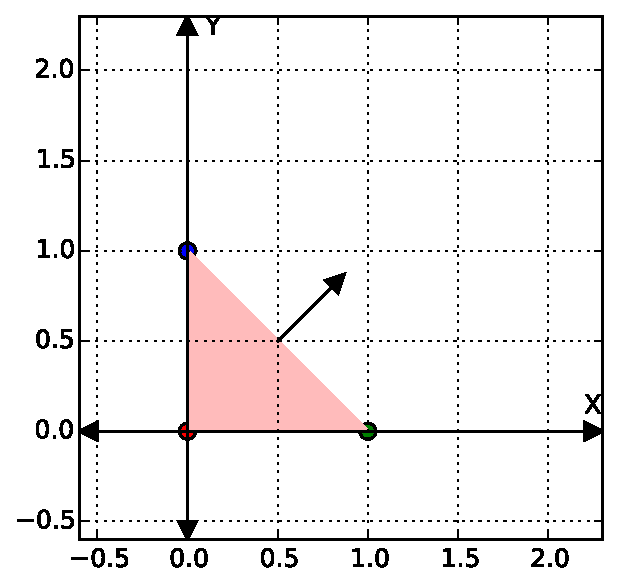
\includegraphics[width=0.46\textwidth]{2DTriOrigNormal.pdf}
	}
	\subfloat[After]{
	    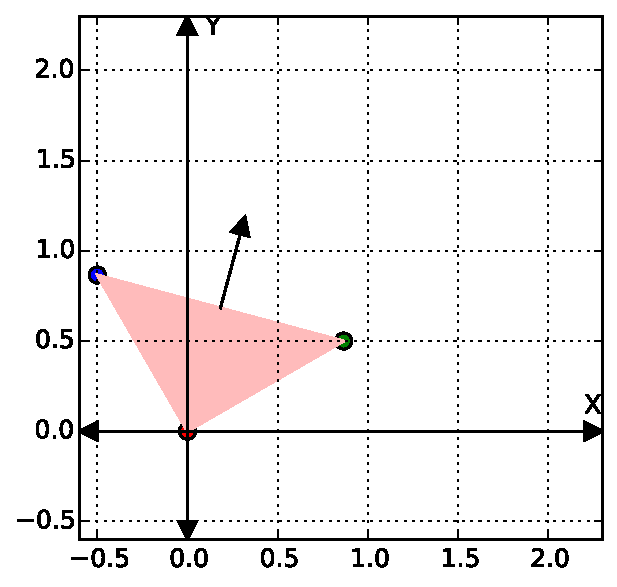
\includegraphics[width=0.46\textwidth]{2DRotateNormal.pdf}
	}
\end{figure}

\end{frame}


\begin{frame}{Normal Transformations}

\uncover<2->{\textcolor{red}{Uh oh....}}

\[ \left[ \begin{array}{cc} 2 & 0\\ 0 & 1\end{array} \right] \left[ \begin{array}{c} x \\ y \end{array} \right] =  \left[ \begin{array}{c} 2x\\ y \end{array} \right] \]

\begin{figure}[t]
    \captionsetup[subfloat]{labelformat=empty}
	\centering
	\subfloat[Before]{
	    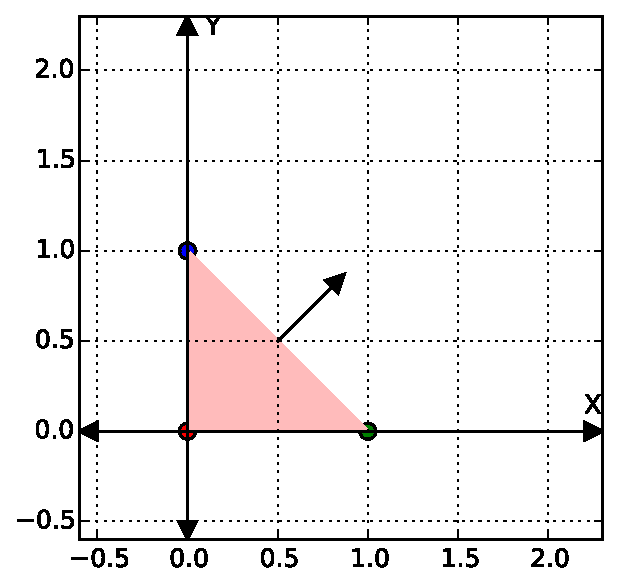
\includegraphics[width=0.46\textwidth]{2DTriOrigNormal.pdf}
	}
	\subfloat[After]{
	    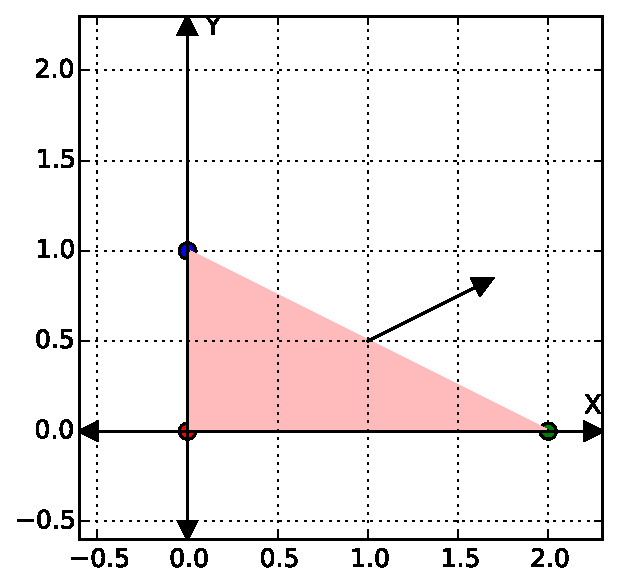
\includegraphics[width=0.46\textwidth]{2DScaleXNormal.pdf}
	}
\end{figure}

\end{frame}


\begin{frame}{Normal Transformation Corrected}

\begin{figure}[t]
    \centering
	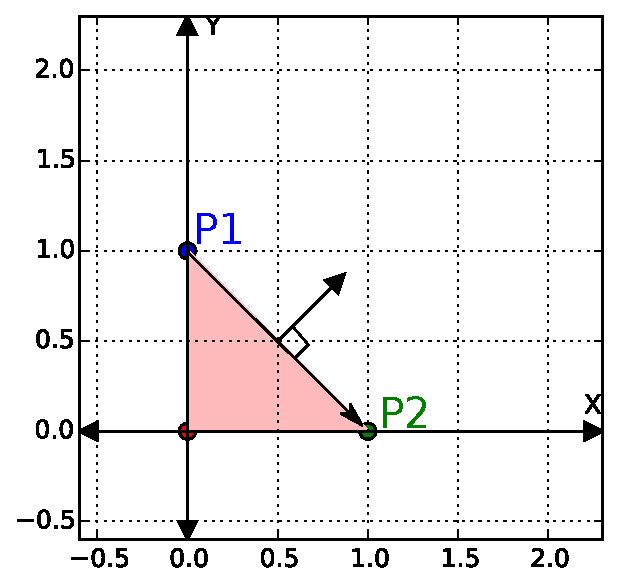
\includegraphics[width=0.4\textwidth]{2DTriTangent.pdf}
\end{figure}

\[ \text{Tangent Vector:} \vec{T} = \vec{P_2} - \vec{P_1} \]

\[ \text{Normal Vector:} \vec{N} \]

Treating as column vectors: $ T^T N = 0$

\end{frame}


\begin{frame}{Normal Transformation Corrected}
Given Transformation matrix $A$, transformed tangent vector is

\[ AP_2 - AP_1 = A(P_2-P_1) = AT\]

\uncover<2->{
Want to find a matrix $G$ s.t. transformed normal $GN$ is orthogonal to $AT$

\[ (AT)^T(GN) = 0 \]

}

\end{frame}


\begin{frame}{Normal Transformation Corrected}

\[ (AT)^T(GN) = 0 \]

\uncover<2->{

\[ T^TA^TGN = 0 \]

}

\uncover<3->{

\[ T^T(A^TG)N = 0 \]

}

\uncover<4->{
We know $T^TN = 0$, so $A^TG = I$

}

\uncover<4->{
Therefore, $G = (A^T)^{-1}$

}


\end{frame}

\begin{frame}{Normal Transformation Corrected}
\[ A = \left[ \begin{array}{cc} 2 & 0\\ 0 & 1\end{array} \right], G = (A^T)^{-1} = A^{-1} = \left[ \begin{array}{cc} 0.5 & 0\\ 0 & 1 \end{array} \right] \]

\begin{figure}[t]
    \captionsetup[subfloat]{labelformat=empty}
	\centering
	\subfloat[Before]{
	    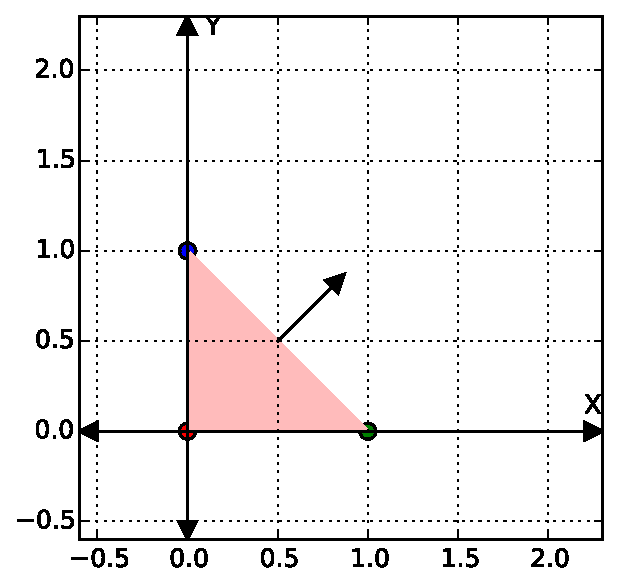
\includegraphics[width=0.46\textwidth]{2DTriOrigNormal.pdf}
	}
	\subfloat[After]{
	    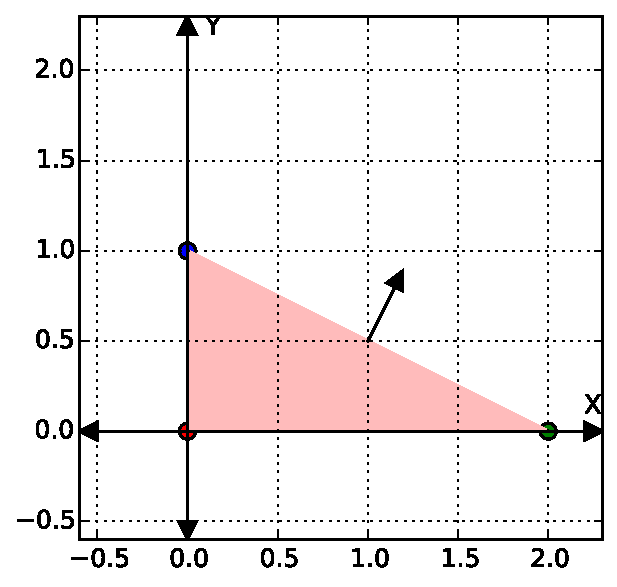
\includegraphics[width=0.46\textwidth]{2DScaleXNormalCorrect.pdf}
	}
\end{figure}

\end{frame}

\begin{frame}{Normal Transformations Corrected}

\[ A = \left[ \begin{array}{cc} \cos(\theta) & -\sin(\theta)\\ \sin(\theta) & \cos(\theta) \end{array} \right], G = (A^T)^{-1} = (A^{-1})^{-1} = A \]

\begin{figure}[t]
    \captionsetup[subfloat]{labelformat=empty}
	\centering
	\subfloat[Before]{
	    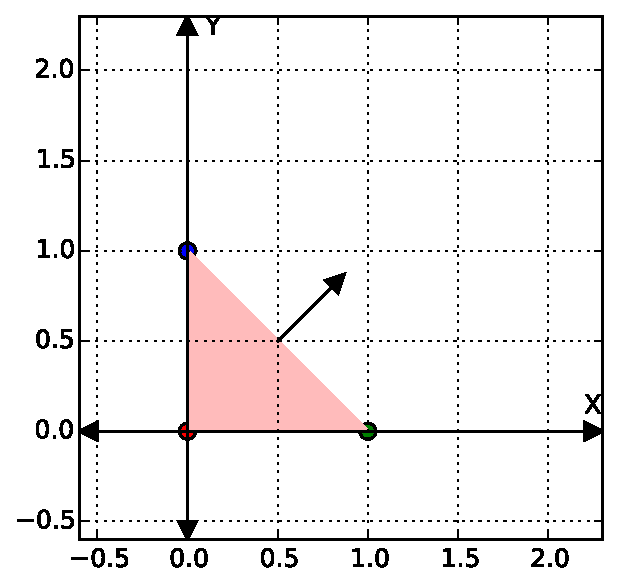
\includegraphics[width=0.46\textwidth]{2DTriOrigNormal.pdf}
	}
	\subfloat[After]{
	    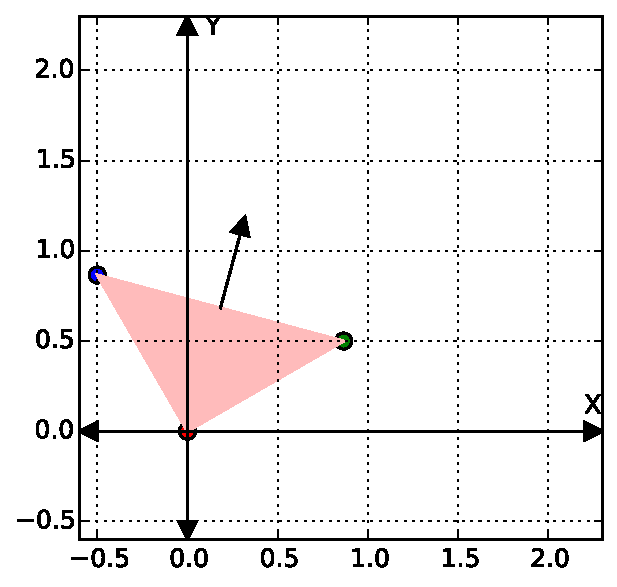
\includegraphics[width=0.46\textwidth]{2DRotateNormal.pdf}
	}
\end{figure}

\end{frame}


\begin{frame}{Normal Transformations Corrected}

\[ A = \left[ \begin{array}{cc} \frac{3}{2} & 1 \\ 0 & 1 \end{array} \right], G = (A^T)^{-1} =  \left[ \begin{array}{cc} \frac{2}{3} & 0 \\ -\frac{2}{3} & 1 \end{array} \right] \]

\begin{figure}[t]
    \captionsetup[subfloat]{labelformat=empty}
	\centering
	\subfloat[Before]{
	    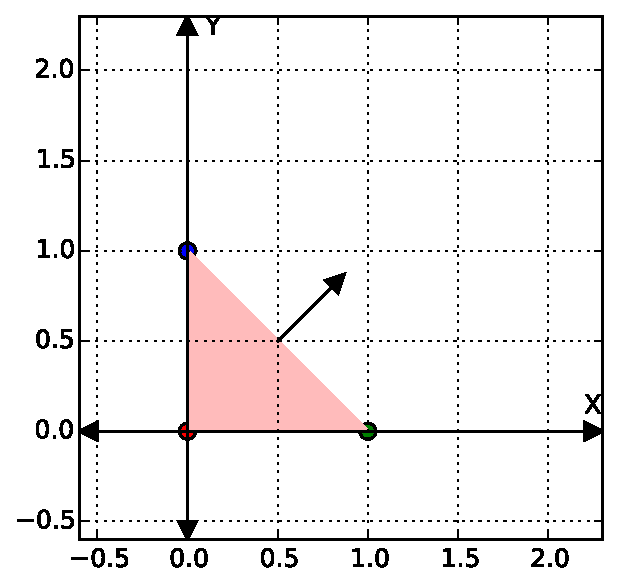
\includegraphics[width=0.46\textwidth]{2DTriOrigNormal.pdf}
	}
	\subfloat[After]{
	    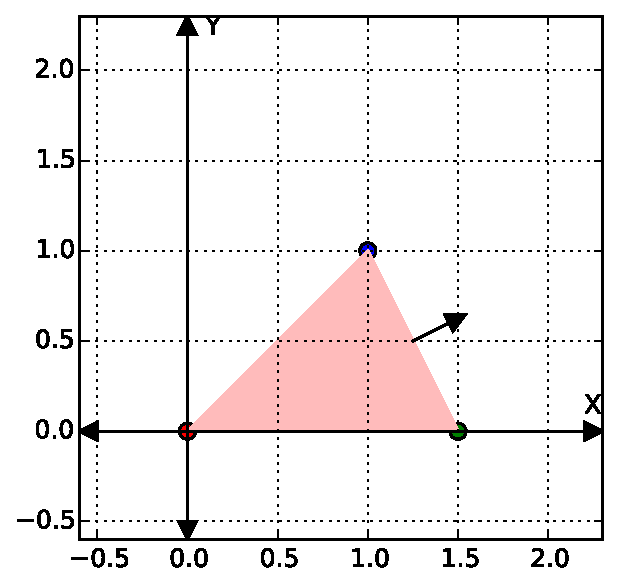
\includegraphics[width=0.46\textwidth]{2DScaleSkewNormal.pdf}
	}
\end{figure}

\end{frame}


\begin{frame}{Table of Contents}

\begin{itemize}[label=$\vartriangleright$]
	\item Linear Functions Continued
	\item Normal Transformations
\end{itemize}
\begin{itemize}[label=$\blacktriangleright$]
	\item Linear Equations
\end{itemize}

\begin{itemize}[label=$\vartriangleright$]
    \item 3D Transformations / Euler Angles
\end{itemize}

\end{frame}


\begin{frame}{Linear Equations Geometric Interpretation}

\[Ax = b \]

\[ \left[ \begin{array}{cc} \textcolor{blue}{\vec{v1}} & \textcolor{red}{\vec{v2}} \end{array} \right] \left[ \begin{array}{c} \textcolor{blue}{s} \\ \textcolor{red}{t} \end{array} \right] = \textcolor{magenta}{\vec{b}} \]

\begin{figure}[t]
	\centering
    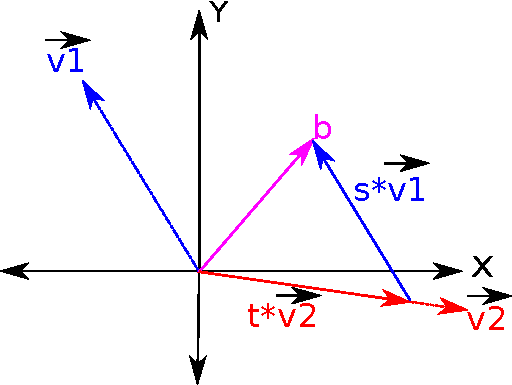
\includegraphics[width=0.6\textwidth]{LinearEquationGeometric.pdf}
\end{figure}


\end{frame}

\begin{frame}{Linear Equations Geometric Interpretation}

\[Ax = b \]

What if $A$ has more rows than columns?

\begin{figure}[t]
	\centering
    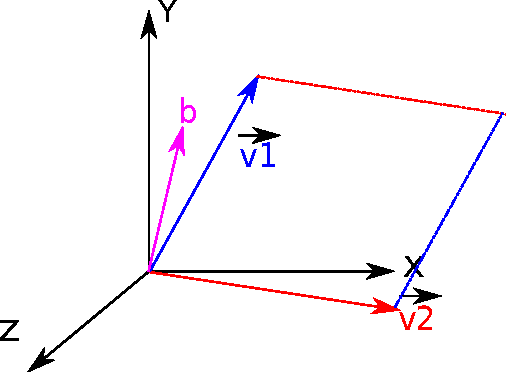
\includegraphics[width=0.5\textwidth]{LinearEquationGeometricOver.pdf}
\end{figure}


\end{frame}

\begin{frame}{Linear Equations Geometric Interpretation}

\[Ax = b \]

What if $A$ has more rows than columns?

\[ (A^TA)x = (A^Tb) \]

\begin{figure}[t]
	\centering
    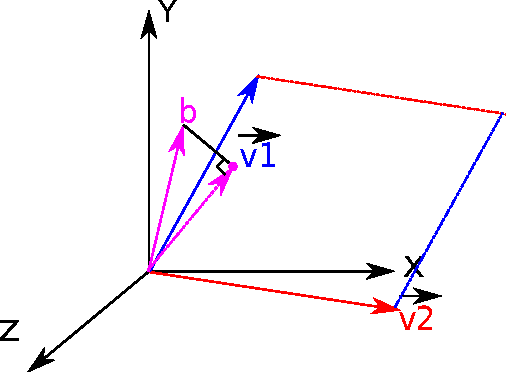
\includegraphics[width=0.5\textwidth]{LinearEquationGeometricOverProj.pdf}
\end{figure}

Least Squares solution / Pseudoinverse

\end{frame}


\begin{frame}{Table of Contents}

\begin{itemize}[label=$\vartriangleright$]
	\item Linear Functions Continued
	\item Normal Transformations
	\item Linear Equations
\end{itemize}

\begin{itemize}[label=$\blacktriangleright$]
    \item 3D Transformations / Euler Angles
\end{itemize}

\end{frame}

\begin{frame}{3D Scale X}

\[ \left[ \begin{array}{ccc} 2 & 0 & 0\\ 0 & 1 & 0 \\ 0 & 0 & 1 \end{array} \right] \left[ \begin{array}{c} x \\ y \\ z \end{array} \right] =  \left[ \begin{array}{c} 2x \\ y \\ z \end{array} \right] \]

\begin{figure}[t]
    \captionsetup[subfloat]{labelformat=empty}
	\centering
	\subfloat[Before]{
	    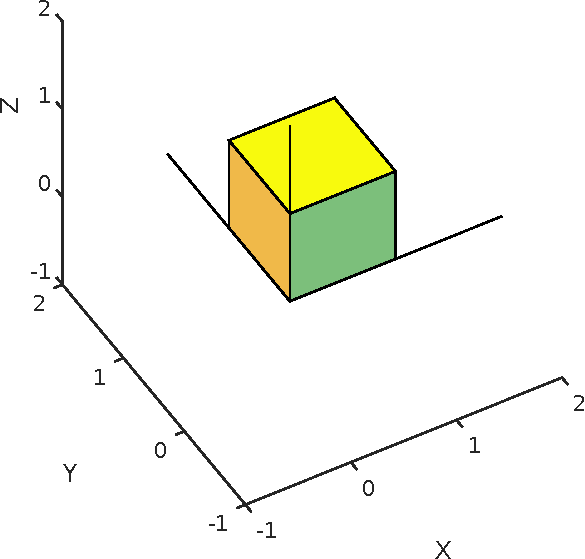
\includegraphics[width=0.46\textwidth]{CubeOrig.pdf}
	}
	\subfloat[After]{
	    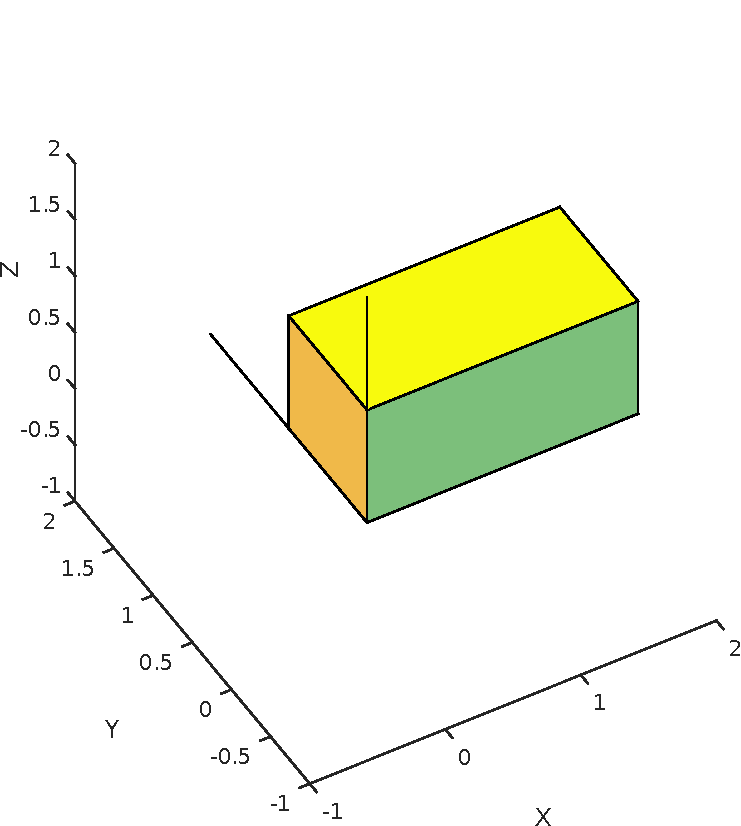
\includegraphics[width=0.46\textwidth]{ScaleX.pdf}
	}
\end{figure}

\end{frame}


\begin{frame}{3D Flip XZ}

\[ \left[ \begin{array}{ccc} -1 & 0 & 0\\ 0 & 1 & 0 \\ 0 & 0 & -1 \end{array} \right] \left[ \begin{array}{c} x \\ y \\ z \end{array} \right] =  \left[ \begin{array}{c} -x \\ y \\ -z\end{array} \right] \]

\begin{figure}[t]
    \captionsetup[subfloat]{labelformat=empty}
	\centering
	\subfloat[Before]{
	    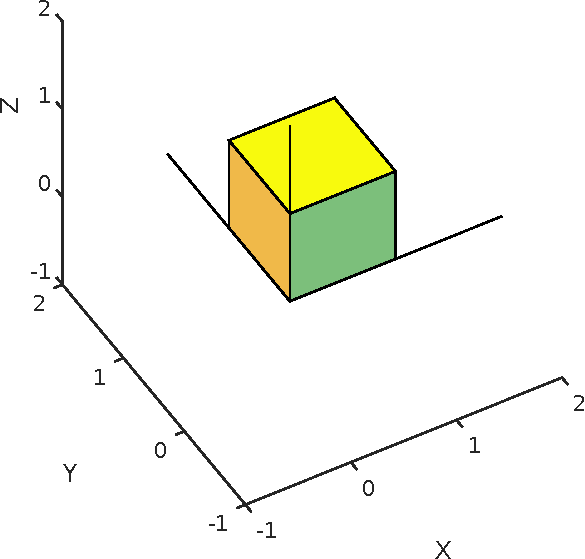
\includegraphics[width=0.46\textwidth]{CubeOrig.pdf}

	}
	\subfloat[After]{
	    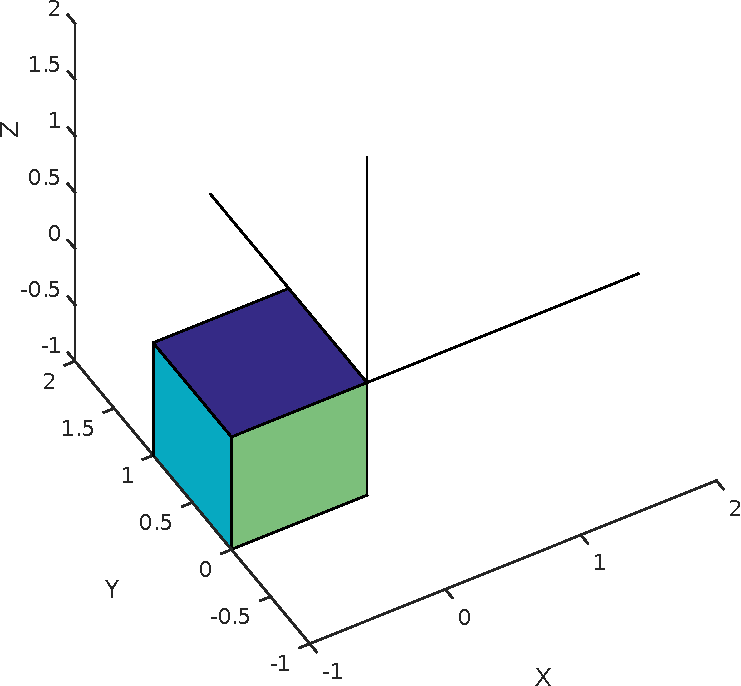
\includegraphics[width=0.46\textwidth]{FlipXZ.pdf}
	}

\end{figure}

\end{frame}

\begin{frame}{X Shear Along Y}

\[ \left[ \begin{array}{ccc} 1 & 1 & 0\\ 0 & 1 & 0 \\ 0 & 0 & 1 \end{array} \right] \left[ \begin{array}{c} x \\ y \\ z \end{array} \right] =  \left[ \begin{array}{c} x + y \\ y \\ z \end{array} \right] \]

\begin{figure}[t]
    \captionsetup[subfloat]{labelformat=empty}
	\centering
	\subfloat[Before]{
	    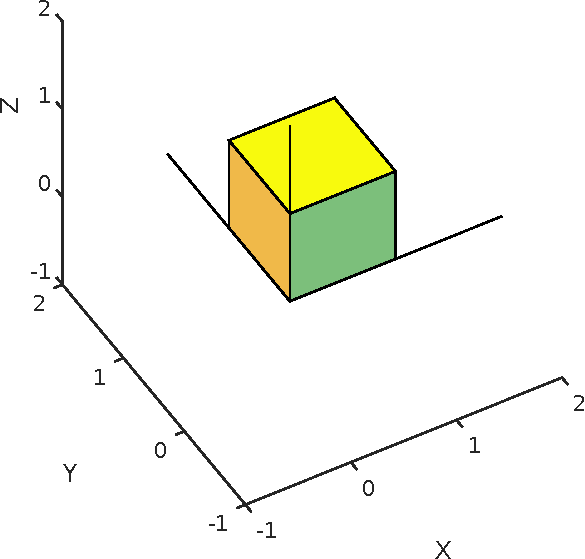
\includegraphics[width=0.46\textwidth]{CubeOrig.pdf}
	}
	\subfloat[After]{
	    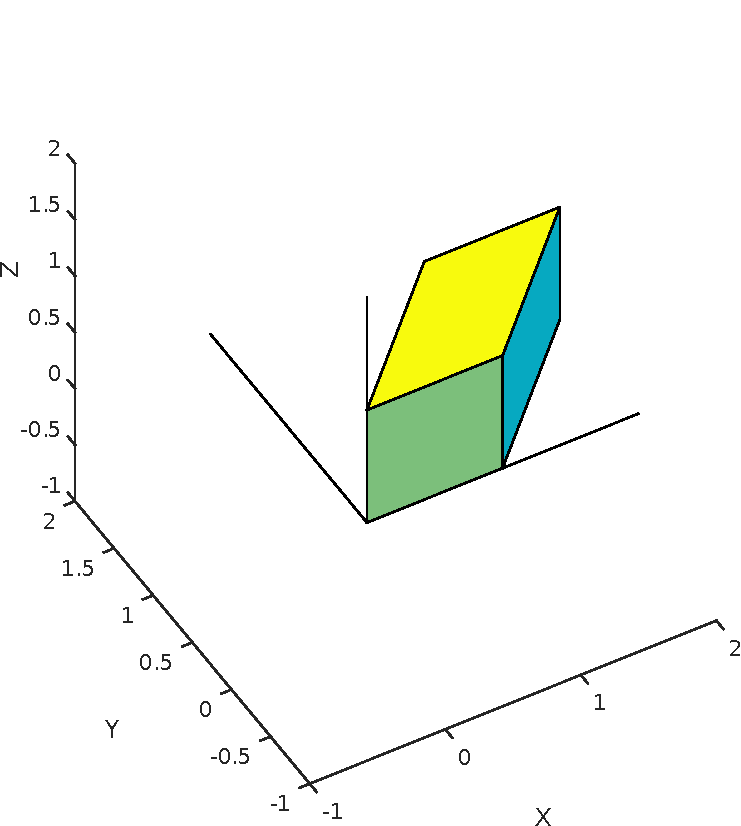
\includegraphics[width=0.46\textwidth]{ShearX.pdf}
	}

\end{figure}
\end{frame}

\begin{frame}{X Shear Along Y and Z}

\[ \left[ \begin{array}{ccc} 1 & 1 & 1\\ 0 & 1 & 0 \\ 0 & 0 & 1 \end{array} \right] \left[ \begin{array}{c} x \\ y \\ z \end{array} \right] =  \left[ \begin{array}{c} x + y + z \\ y \\ z \end{array} \right] \]

\begin{figure}[t]
    \captionsetup[subfloat]{labelformat=empty}
	\centering
	\subfloat[Before]{
	    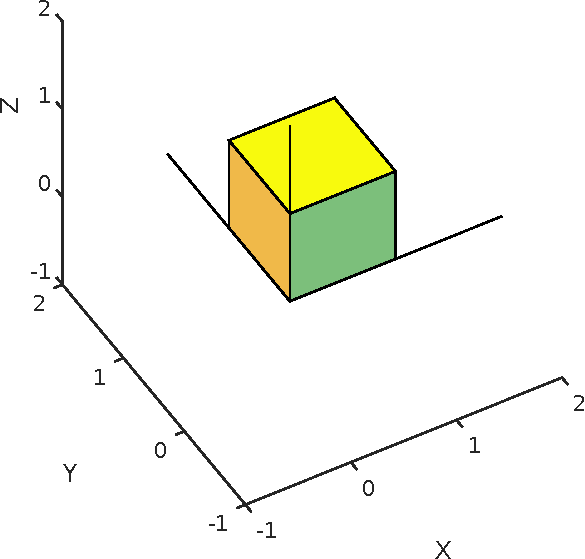
\includegraphics[width=0.46\textwidth]{CubeOrig.pdf}
	}
	\subfloat[After]{
	    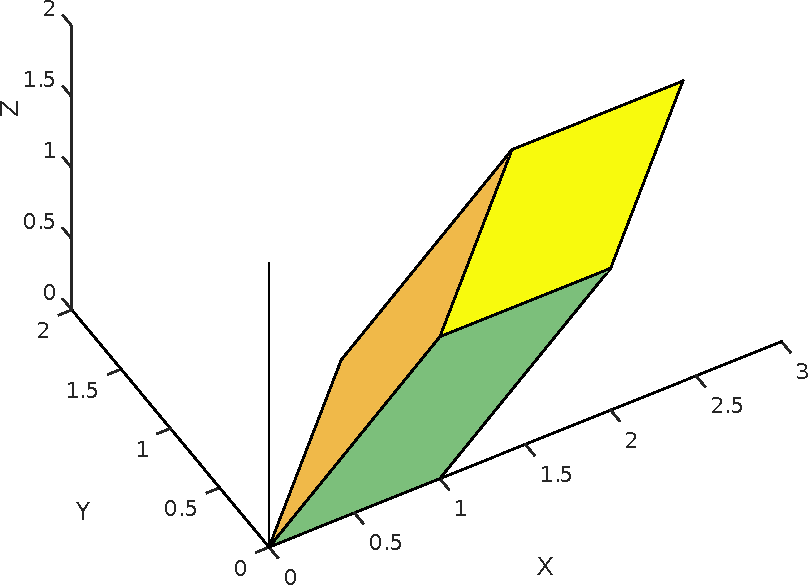
\includegraphics[width=0.46\textwidth]{DoubleShearX.pdf}
	}

\end{figure}

\end{frame}


\begin{frame}{X Shear Along Y, Y Shear Along Z}

\[ \left[ \begin{array}{ccc} 1 & 1 & 0\\ 0 & 1 & 1 \\ 0 & 0 & 1 \end{array} \right] \left[ \begin{array}{c} x \\ y \\ z \end{array} \right] =  \left[ \begin{array}{c} x + y \\ y + z \\ z \end{array} \right] \]

\begin{figure}[t]
    \captionsetup[subfloat]{labelformat=empty}
	\centering
	\subfloat[Before]{
	    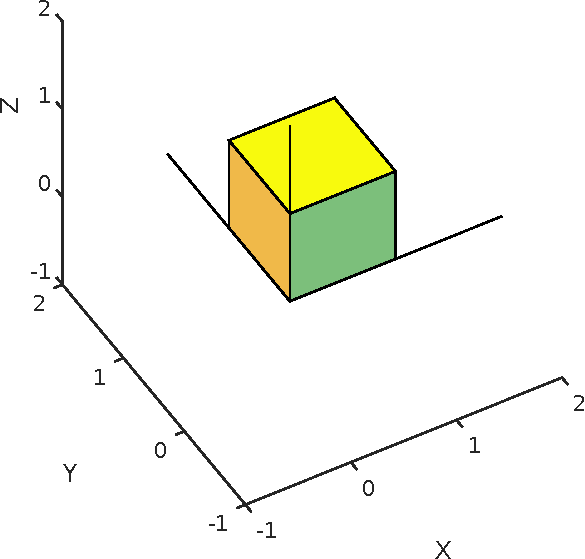
\includegraphics[width=0.46\textwidth]{CubeOrig.pdf}
	}
	\subfloat[After]{
	    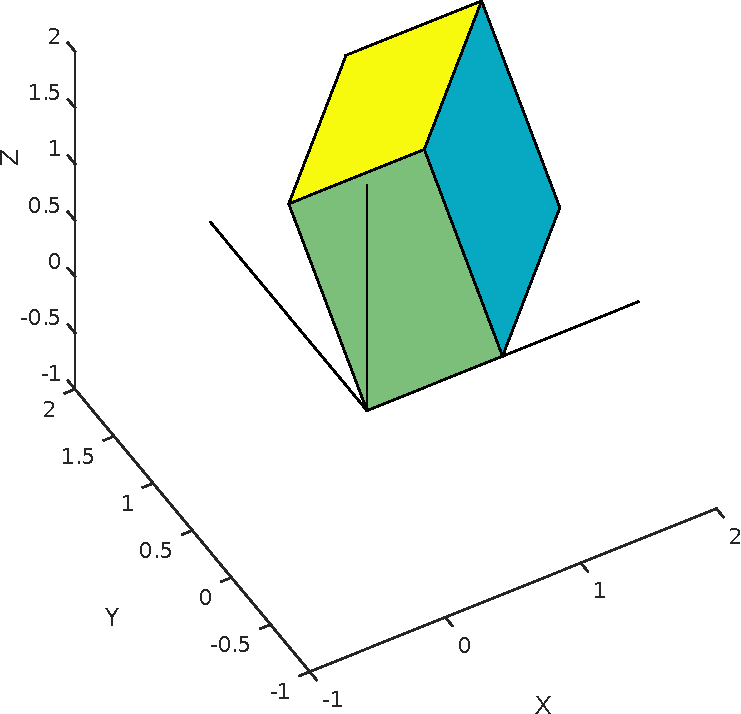
\includegraphics[width=0.46\textwidth]{ShearXY.pdf}
	}

\end{figure}

\end{frame}

\begin{frame}{X Shear Along Y, Y Shear Along Z}

\[ \left[ \begin{array}{ccc} 1 & 1 & 0\\ 0 & 1 & 1 \\ 0 & 0 & 1 \end{array} \right] \left[ \begin{array}{c} x \\ y \\ z \end{array} \right] =  \left[ \begin{array}{c} x + y \\ y + z \\ z \end{array} \right] \]

Interactive Demo

\end{frame}


\begin{frame}{3D Homogenous Coordinates}

\[ A = \left[
\begin{array}{cccc}
A_{11} & A_{12} & A_{13} & T_x \\
A_{21} & A_{22} & A_{23} & T_y \\
A_{31} & A_{32} & A_{33} & T_z \\ 
0 & 0 & 0 & 1
\end{array}
\right]
\]

\uncover<2->{
\[
A \left[ \begin{array}{c} x \\ 1 \end{array} \right] = \left[ \begin{array}{c} A^{3 \times 3}x + \left[ \begin{array}{c} T_x \\ T_y \\ T_z \end{array} \right] \\ 1 \end{array} \right]
\]
}

\end{frame}

\begin{frame}{2D Rotation Matrix Design: Review}

\begin{figure}[t]
	\centering
    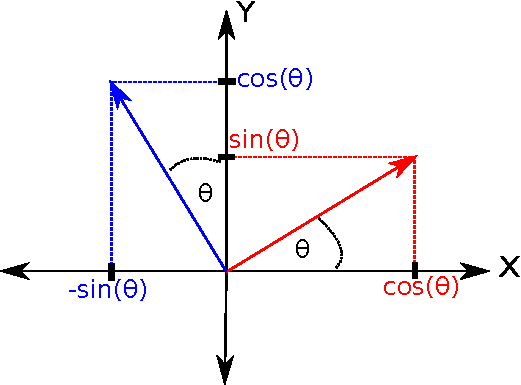
\includegraphics[width=0.6\textwidth]{ColumnVectorRot2.pdf}
\end{figure}


\[ \left[ \begin{array}{cc} \textcolor{red}{\cos(\theta)} & \textcolor{blue}{-\sin(\theta)} \\ \textcolor{red}{\sin(\theta)} & \textcolor{blue}{\cos(\theta)} \end{array}  \right] \]

\end{frame}

\begin{frame}{Rotation About X}

\[ R_X(\gamma) = \left[ \begin{array}{ccc} \textcolor{blue}{1} & \textcolor{red}{0} & \textcolor{darkgreen}{0} \\ \textcolor{blue}{0} & \textcolor{red}{\cos(\gamma)} & \textcolor{darkgreen}{-\sin(\gamma)}  \\ \textcolor{blue}{0} & \textcolor{red}{\sin(\gamma)} & \textcolor{darkgreen}{\cos(\gamma)} \end{array}\right] \]

\begin{figure}[t]
	\centering
	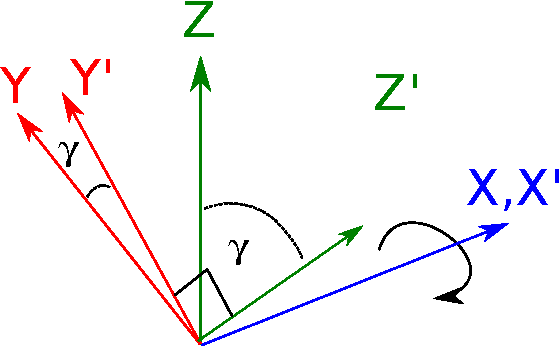
\includegraphics[width=0.6\textwidth]{3DRotX.pdf}
\end{figure}

\end{frame}


\begin{frame}{Rotation About Y}

\[ R_Y(\beta) = \left[ \begin{array}{ccc} \textcolor{blue}{\cos(\beta)} & \textcolor{red}{0} & \textcolor{darkgreen}{\sin(\beta)} \\ \textcolor{blue}{0} & \textcolor{red}{1} & \textcolor{darkgreen}{0}  \\ \textcolor{blue}{-\sin(\beta)} & \textcolor{red}{0} & \textcolor{darkgreen}{\cos(\beta)} \end{array}\right] \]

\begin{figure}[t]
	\centering
	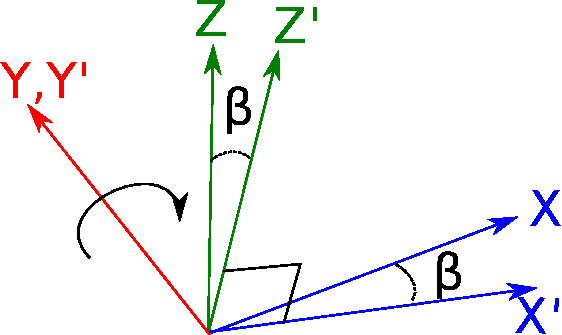
\includegraphics[width=0.6\textwidth]{3DRotY.pdf}
\end{figure}

This one hurts the brain a little

\end{frame}

\begin{frame}{Rotation About Z}

\[ R_Z(\alpha) = \left[ \begin{array}{ccc} \textcolor{blue}{\cos(\alpha)} & \textcolor{red}{-\sin(\alpha)} & \textcolor{darkgreen}{0} \\ \textcolor{blue}{\sin(\alpha)} & \textcolor{red}{\cos(\alpha)} & \textcolor{darkgreen}{0}  \\ \textcolor{blue}{0} & \textcolor{red}{0} & \textcolor{darkgreen}{1} \end{array}\right] \]

\begin{figure}[t]
	\centering
	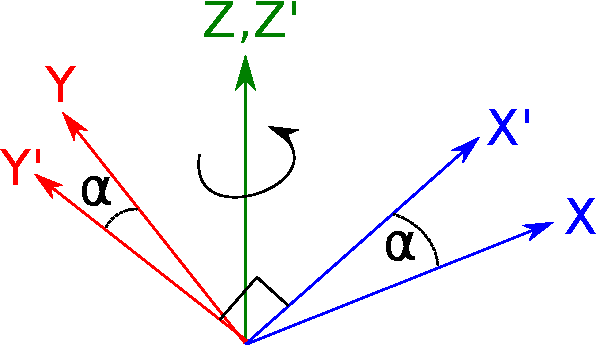
\includegraphics[width=0.6\textwidth]{3DRotZ.pdf}
\end{figure}

Just like the normal 2D $XY$ rotation

\end{frame}

\begin{frame}{Euler Angles}

Can chain these matrices together in any order, such as

\[ R_{ZYX} = R_X(\gamma) R_Y(\beta) R_Z(\alpha) \]

\[ R_{XYZ} = R_Z(\alpha) R_Y(\beta) R_X(\gamma)  \]

Resulting matrix is always \em{orthogonal}

\end{frame}

\begin{frame}{Euler Angles: Raffle Point Question}

\uncover<2->{
How many degrees of freedom to reach any 3D orientation? Give me a reason
}

\uncover<3->{
\begin{itemize}[label=$\vartriangleright$]
\item Each column of the matrix is a unit vector
\end{itemize}
}

\uncover<4->{
\begin{itemize}[label=$\vartriangleright$]
\item Every pair of columns is orthogonal.   \\
In matrix language, $A^TA = I$
\end{itemize}
}

\end{frame}

\begin{frame}{Euler Angles}

Euler Angles Demo

\end{frame}

%\begin{frame}{Projections}

%\[ \frac{f}{u} = \frac{y}{x} \implies u = f \left( \frac{y}{x} \right) \]

%\begin{figure}[t]
%	\centering
%	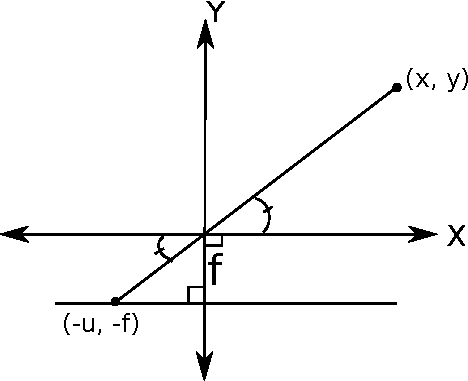
\includegraphics[width=0.6\textwidth]{Projection.pdf}
%\end{figure}

%\end{frame}

\end{document}

